\chapter{Efficient Solution Algorithms: Iterative methods and Preconditioning}

To compute the solution of a partial differential equation, we often 
need to solve a system of linear of equations with a large number of
uknowns. The accuracy of the solution increase with 
the number of unknowns used. Nowadays,  unknowns in the order
of millions to billions are routinely solved for  without the use of (state-of-the-art) 
high-performance computing. Such computations
are fasilitated by the enormous improvements in numerical algorithms and
scientific software the last decades.        

It should be quite clear that naive Gaussian elimination can not be employed. 
For a  naive Gaussian eliminations implementaton,   
the number of required floating point operations (FLOPS) scales as the cube
of the number of uknowns. Hence, solving a problem with $10^6$ unknowns
would then require $10^{18}$ FLOPS which on a modern computer
with e.g. 3 GHz still would take about 10 years. As we will see later, 
such problems may in common cases be solved in just a few seconds.  
There are two ingrediences in such efficient algorithms: 
{\it iterative methods} and {\it preconditioning}. 

%Pre text
Lets therefore consider the numerical solution of large linear systems,
\[
A u =  b,
\]
where the linear system comes from discretization of PDEs. That is,  
$A$ is a $N\times N$ matrix, and $N$ is between $10^6$ and $10^9$ 
in typical simulations. Furthermore, the matrix is normally extremely sparse and contains only $\mathcal{O}(N)$ 
nonzeros (see Exercise \ref{ex:nnz}). It is important to notice that 
even though $A$ is sparse $A^{-1}$ will in general be full. 
This is a main reason to consider iterative methods. 

%------------------------------------------------------------------------------
\section{The simplest iterative method: the Richardson iteration}
\index{Richardson iteration}
The Richardson iteration\footnote{
Richardson developed his method prior to computers. 
In his 1910 paper, where the focus is to predict stresses in a masonry dam, he 
describes how he uses humans as computational resources.  
He writes "So far I have paid piece rates for
the operation [Laplacian] of about $n/18$ pence per coordinate point, $n$
being the number of digits. As for the rate of working, one of the quickest 
boys average 2000 operations per week, for numbers of three digits, those
done wrong being discounted."}    is  
\begin{equation}
\label{eq:Richardson_simple}
u^n = u^{n-1} - \tau (A u^{n-1} - b),
\end{equation}
where $\tau$ is a relaxation parameter that must be determined.
Clearly, the method is consistent in the sense that  
if $u^{n-1} = u$, then $u^{n} = u$ and the iterative method has converged to 
the exact solution. It is also clear that each iteration requires the evaluation of $A$ on a vector, in 
addition to vector addition and scalar multiplication. Hence, one iteration requires
the amount of  $\mathcal{O}(N)$ FLOPS and only $\mathcal{O}(N)$ 
of memory. This is a dramatic improvement when compared Gaussian elimination at least if  
if the number of iterations are few. The key to obtain few iterations is 
preconditioning, but lets first consider the Richardson's method without.     
\\

The standard approach to analyze iterative methods is to look at what happens with the \textit{error}.
Let the error at the $n$'th iteration be  
$e^n = u^n -u$. As this is a linear system of equations, we may subtract $u$ from both sides of (\ref{eq:Richardson_simple}) 
and obtain an equation for the iterative error: 
\[
e^n = e^{n-1} - \tau A e^{n-1} .
\]
We may therefore quantify the error in terms of the $L^2$-norm as
\[
\Vert e^n \Vert = \Vert e^{n-1} - \tau A e^{n-1} \Vert \le \Vert I - \tau A \Vert \Vert e^{n-1}\Vert .  
\]
Clearly, if $\Vert I - \tau A \Vert < 1$ then the iteration will be convergent. 
\\

Assuming for the moment that $A$ is symmetric and positive definite, then  
the norm of $A$ in general defined as 
\[
\Vert A\Vert = \max_x \frac{\Vert Ax \Vert}{\Vert x \Vert} 
\]
equals the largest eigenvalue of $A$, $\lambda_{max}$.   
Furthermore, if we assume that the eigenvalues are ordered with respect to increasing value,
such that  $\lambda_0$ and $\lambda_N$ are the smallest and largest eigenvalue, then the
norm of $I - \tau A $, 
\[
\Vert I - \tau A\Vert = \max_x \frac{\Vert (I - \tau A) x \Vert}{\Vert x \Vert} 
\]
is attained either for the smallest or largest eigenvalue as either   
$(1 - \tau \lambda_0)$ or  $-(1 - \tau \lambda_N)$.  
The optimal relaxation parameter $\tau_{opt}$ can be stated in terms of the eigenvalues,    $\lambda_i$,  of $A$. 
Minimum is attained
when $(1 - \tau_{opt} \lambda_0) = -(1 - \tau_{opt} \lambda_N)$ which makes   
$\tau_{opt} = \frac{2}{\lambda_0 + \lambda_N}$.

Let the convergence factor $\rho$ be defined as 
\[
\rho = \Vert I - \tau A\Vert 
\]
The convergence factor with an optimal relation is then 
\[
\rho = \Vert I - \tau A\Vert = \max_{\lambda_i}\vert 1- \tau \lambda_i\vert  = 
1 - \tau\lambda_0 = 1 - \frac{2\lambda_0}{\lambda_0 + \lambda_N} = 
\frac{\lambda_N - \lambda_0}{\lambda_N + \lambda_0} = \frac{\kappa - 1}{\kappa + 1}.
\]  
Here, $\kappa=\frac{\lambda_N}{\lambda_0}$ is the condition number. 

We estimate the error reduction per iteation in terms of the convergence factor as, 
\[
\Vert e^n \Vert = \Vert (I - \tau A) e^{n-1} \Vert \le  \rho \Vert e^{n-1}\Vert .  
\]
which leads to
\[
\Vert e^n \Vert \le (\frac{\kappa - 1}{\kappa + 1})^n\Vert e^0\Vert. 
\]


For iterative methods, we never iterate until the true solution exactly. Instead a convergence 
criteria needs to be choosen such that the error obtained by the iterative method is
less than or at least comparable to the approximation error of the original system.      
Determining an appropriate convergence criteria is problem dependent and quite often 
challenging. 

Nevertheless, let us assume  that we need to reduce the error by a factor of $\epsilon$, 
that is, we need $\frac{\Vert e^n\Vert}{\Vert e^0 \Vert} < \epsilon$. From the iteration, we have 
\begin{equation}
\label{eq:convergence}
\Vert e^n \Vert \le \rho \Vert e^{n-1} \Vert \le \rho^n \Vert e^0 \Vert.
\end{equation}

An estimate for the number of iterations is then obtained by assuming
equality in the equation (\ref{eq:convergence}) and $\frac{\Vert e^n\Vert}
{\Vert e^0 \Vert} = \epsilon$. Then the number of iterations needed to achieve the 
desired error is:
\begin{equation}
\label{no_iterations}
n = \frac{\log \epsilon}{\log \rho} = \frac{\log \epsilon}{\log (\frac{K-1}{K+1})} .
\end{equation} 
If $n$ is independent of the resolution of the discretization, the computational cost of the algorithm is  $\mathcal{O}(N)$ in FLOPS and memory 
and the algorithm is \textit{order-optimal}. \\

The current analysis of the simplest iterative method there is, the Richardson iteration,  shows that the efficiency of the method 
is determined by the condition number of the matrix. In the literature you will find a jungle of
methods of which the following are the most famous: the Conjugate Gradient method, the Minimal Residual method, the BiCGStab method, and the GMRES method.  It is remarkable that in general the convergence of these methods is determined by the condition number with one exception; the Conjugate Gradient method which often can be estimated in terms of the square root of the condition number. One main advantage is however that these methods
do not require the determination of a $\tau$ to obtain convergence.    

\begin{example}{\textbf{Eigenvalues of an elliptic problem in 1D and 2D.}} \\
Let us consider an elliptic problem: 
\begin{eqnarray}
u - \Delta u &=& f, \quad \text{ in } \Omega, \\     
\frac{\partial u}{\partial n} &=& 0, \quad \text{ on } \partial \Omega .  
\end{eqnarray}
Notice that the lower order term $u$ in front of $-\Delta u$ makes removes
the singularity associated with Neumann conditions and that in the continuous
case the smallest eigenvalue is 1 (associated with the eigenfunction that is a constant throughout $\Omega$). 
The following code computes the eigenvalues using 
linear Lagrangian elements and  
\begin{python}
from dolfin import *
from numpy import linalg 

for D in [1, 2]: 
  for N in [4, 8, 16, 32]:
    if   D == 1:  mesh = UnitIntervalMesh(N)
    elif D == 2:  mesh = UnitSquareMesh(N, N)

    V = FunctionSpace(mesh, "Lagrange", 1)
    u = TrialFunction(V)
    v = TestFunction(V)

    a = u*v*dx  + inner(grad(u), grad(v))*dx  
    A = assemble(a) 
    e = linalg.eigvals(A.array()) 
    e.sort()
    c = e[-1] / e[0]

    print "D=\%d, N=\%3d, min eigenvalue=\%5.3f, max eigenvalue=\%5.3f, cond. number=\%5.3f " \% (D, N, e[0], e[-1], c) 
\end{python}
yields the following output:  
\terminal{
D=1, N=  4, min eig=0.199, max eig=14.562,  cond. number=73.041 \\ 
D=1, N=  8, min eig=0.111, max eig=31.078,  cond. number=279.992 \\  
D=1, N= 16, min eig=0.059, max eig=63.476,  cond. number=1079.408 \\ 
D=1, N= 32, min eig=0.030, max eig=127.721, cond. number=4215.105 \\ 
D=2, N=  4, min eig=0.040, max eig=7.090,   cond. number=178.444 \\  
D=2, N=  8, min eig=0.012, max eig=7.735,   cond. number=627.873 \\  
D=2, N= 16, min eig=0.003, max eig=7.929,   cond. number=2292.822 \\  
D=2, N= 32, min eig=0.001, max eig=7.982,   cond. number=8693.355 \\ 
}
The output shows that the condition number grows as $h^{-2}$ in both 1D and 2D although
the behaviour of the eigenvalues clearly are dimension dependent (see Exercise \ref{ex:eig:1D2D3D}). The smallest eigenvalue decrease in both 1D and 2D as $h\rightarrow 0$ but at different rates. To obtain eigenvalues corresponding the
true eigenvalue we would need to solve a generalized eigenvalue problem 
as discussed in Chapter \ref{chap-sobolev}.           
\end{example}


\begin{example}{\textbf{The Richardson iteration applied to a  1D Poisson equation.}}\label{ex:1D_poisson}\\ %endline
The Richardson iteration on the Poisson equation in 1D, discretized with finite difference method (FDM).
\begin{align}
Lu =&\left\{ \begin{array}{lr}  -u'' = f \quad \text{for} \quad x \in (0,1)\\ 
u(0) = u(1) = 0  \end{array} \right.
\end{align}
Eigenvalues and eigenfunctions of $Lu$ are $\lambda_k = (k\pi)^2$ and $v_k = \sin(k\pi x) $ 
for $k \in \mathbb{N}$. 
When discretizing with FDM we get a $Au = b$ system, where $A$ is a tridiagonal matrix
($A = \text{tridiagonal}(-1,2,-1)$) when the Dirichlet conditions have
been eliminated. The discrete and continuous eigenvectors are the same, but the eigenvalues are a little 
bit different: $\lambda_{k} = \frac{4}{h^2}sin^2(\frac{k\pi h}{2})$, where $h$ is the step 
lenght $\Delta x$. We find the smallest and largest discrete eigenvalues
\[
\lambda_{min}(A) = \pi^2, \quad \lambda_{max}(A) = \frac{4}{h^2}. 
\]
Let $\tau = \frac{2}{\lambda_{max} + \lambda_{min}}$ then from the analysis above,
\[
\Vert e^n\Vert \le (\frac{1-K}{1+K})^{n}\Vert e^0 \Vert.
\]
The below code perform the Richardson iteration for various 
resolution on the 1D Poisson problem and stops when 
the convergence criteria $\frac{\|r_k\|}{\|r_0\|} \le 10^{-6}$ 
is obtained. 
\begin{python}
from numpy import * 

def create_stiffness_matrix(N): 
  h = 1.0/(N-1)
  A = zeros([N,N])
  for i in range(N): 
    A[i,i] = 2.0/(h**2) 
    if i > 0: 
      A[i,i-1] = -1.0/(h**2) 
    if i < N-1: 
      A[i,i+1] = -1.0/(h**2) 
  A = matrix(A)
  return A 

Ns = [10, 20, 40, 80, 160, 320] 
for N in Ns: 
  A = create_stiffness_matrix(N)              # creating matrix
  x = arange(0, 1, 1.0/(N))
  f = matrix(sin(3.14*x)).transpose()         # right hand side
  u0 = matrix(random.random(N)).transpose()   # initial guess 
  u_prev = u0 

  eigenvalues = sort(linalg.eigvals(A))       # compute eigenvalues and tau 
  lambda_max, lambda_min = eigenvalues[-1],  eigenvalues[0]
  print "lambda_max ", lambda_max, " lambda_min ", lambda_min
  tau = 2/(lambda_max + lambda_min)

  norm_of_residual = 1.0                      # make sure the iteration starts
  no_iterations= 0                        
  while norm_of_residual > 1.0e-6: 
    r = A*u_prev - f                          # compute the residual 
    u = u_prev - tau*r                        # the Richardson iteration 
    u_prev = u                                 
    norm_of_residual = r.transpose()*r        # check for norm of residual 
    no_iterations+=1                          # count no iterations  

  print "N ", N, " number of iterations ", no_iterations
 
\end{python}

\begin{table}[h]
\begin{center}
\begin{tabular}{|c|c|c|c|c|}  \hline
$N $ & $\lambda_{min}$ & $\lambda_{max}$& no. iterations & Estimated FLOPS \\ \hline
10 & 6.6  & 317   & 277 &  11 $10^3$      \\ \hline
20  & 8.1 & 1435  & 1088 & 87 $10^3$     \\ \hline
40  & 8.9 & 6075  &  4580 & 732  $10^3$   \\ \hline
80 & 9.4  & 25*$10^3$ & 20 $10^3$ & 6.4 $10^6$ \\ \hline 
160 & 9.6 & 101*$10^3$ & 84 $10^3$ & 53 $10^6$   \\ \hline  
320 & 9.7 & 407*$10^3$ & 354 $10^3$ & 453 $10^6$ \\ \hline 
\end{tabular}
\caption{The number of iterations of the Richardson iteration for 
solving a 1D Poisson problem. The FLOPS is estimated 
as the number of iterations times four times the number of unknowns, $N$, 
as the matrix is tridiagonal and there is both a matrix vector product (3$N$)
and a vector addtion involved in \eqref{eq:Richardson_simple}. }
\label{Richardson:norms}
\end{center}
\end{table}
We remark that in this example we have initialized the iteration with a random vector because
such a vector contains errors at all frequencies. This is recommended practice when 
trying to estabilish a worst case scenario. Testing the iterative method against a known analytical solution with 
a zero start vector will often only require smooth error to be removed during the iterations and will
therefore underestimate the complications of a real-world problem.   
\end{example}



\subsection{The stopping criteria}
In the Example \ref{ex:1D_poisson}  we 
considered the Richardson iteration applied
to a Poisson problem in 1D. We saw that in order to stop
the iteration we had to choose a stopping criteria. Ideally
we would like to stop when the error was small enough.
The problem is that the error is uknown. 
In fact, since $e^n = u^n - u$ we would be able to compute
the exact solution if the error was known at the $n$'th iteration. 
What is computable is the \textit{residual} at the $n$'th iteration, defined
by 
\[
r^n = A u^n - f .  
\]
It is straightforward to show that 
\[
A e^n = r^n . 
\]
But computing $e^n$ from this relation would require the inversion of
$A$ (which we try to avoid at all cost since it in general is a $\mathcal{O}(N^3)$ procedure). For this reason, the convergence criteria is typically
expressed in terms of some norm of the residual.     
We may bound the $n$'th error as  
\[
\|e^n\| \le \|A^{-1}\| \|r^n\| .   
\]
However, estimating $\|A^{-1}\|$ is in general challenging or 
computationally demanding and therefore usually avoided.   
To summarize, choosing an appropriate stopping criteria 
is in general challenging and in practice the choice has to be tailored
to concrete application at hand by trial and error. 


\section{The idea of preconditioning}
\index{Richardson preconditioner}
The basic idea of preconditioning is to replace 
\[
Au = b
\] 
with 
\[
BAu = Bb. 
\]
Both systems have the same solution (if B is nonsingular). However, $B$ should be 
chosen as a cheap approximation of $A^{-1}$ or at least in such a way 
that $BA$ has a smaller condition number than $A$.   
Furthermore $Bu$ should cost $\mathcal{O}(N)$ operations to evaluate. 
Obviously, the  preconditioner $B=A^{-1}$ would make the condition 
number of $BA$ be one and the Richardson iteration would converge in one iteration.   
However, $B=A^{-1}$ is a very computationally demanding preconditioner.  
We would rather seek preconditioners that are  $\mathcal{O}(N)$ 
in both memory consumption and evaluation. 

The generalized Richardson iteration becomes\\


\begin{equation}
\label{eq:Richardson_generalized}
u^n = u^{n-1} - \tau B(A u^{n-1} - b).
\end{equation}
The error in the $n$-th iteration is 
\[
e^n = e^{n-1} - \tau BAe^{n-1}
\]
and the iteration is convergent if $\Vert I - \tau BA\Vert < 1$.

\subsection{Spectral equivalence and order optimal algorithms} \index{Spectral equivalence}

Previously we stated that a good preconditioner is supposed to be similar to $A^{-1}$. 
The precise (and most practical) property that is required of a preconditioner
is: 
\begin{itemize}
\item
  $B$ should be spectrally equivalent with $A^{-1}$.
\item
  The evaluation of $B$ on a vector, $Bv$, should be $\mathcal{O}(N)$.
\item
  The storage of $B$ should be $\mathcal{O}(N)$.
\end{itemize}



%\paragraph{definition:}
\begin{definition}Two linear operators or matrices $A^{-1}$ and $B$, that are symmetric 
and positive definite are spectral equivalent if:

\begin{equation}\label{eq:spectral_equivalence}%and order optimal algorithm
c_1(A^{-1}v,v) \le (Bv,v) \le c_2(A^{-1}v,v) \quad \forall v
\end{equation}
If $A^{-1}$ and $B$ are spectral equivalent, then the condition number 
of the matrix $BA$ is $\kappa(BA) \le \frac{c_2}{c_1}$.
\end{definition}

If the preconditioner $B$ is spectrally equivalent with $A^{-1}$ 
then the preconditioned  Richardson iteration yields 
and order optimal algorithm.  
To see this, we note that $e^n = (I-\tau BA)e^{n-1}$. We can estimate 
the behavior of $e^n$ by using the A-norm, $\rho_A = \Vert I - \tau BA\Vert_A$. 
Then we get
\[
\Vert e^n\Vert_A \le \rho _A \Vert e^{n-1}\Vert_A.
\]
Hence, if the condition number is independent of the discretization 
then the number of iterations  as estimated earlier in \eqref{no_iterations} 
will be bounded independently of the discretization.  

In general, if $A$ is a discretization of $-\Delta$ on a quasi-uniform mesh  
then both multigrid methods and domain decomposition methods will yield 
preconditioners that are spectrally equivalent with the inverse and close 
to $\mathcal{O}(N)$ in evaluation and storage.  
The gain in using a proper preconditioner may provide speed-up of several
orders of magnitude, see Example \ref{example:CPU_time}.  








\section{Krylov methods and preconditioning}
For iterative methods, any method involving linear iterations  may be written as a Richardson iteration with a preconditioner.
However, iterative methods like Conjugate Gradient method, GMRES, Minimal Residual method, and
BiCGStab, are different. These are nonlinear iterations  where 
for instance the relaxation parameter $\tau$ changes during the iterations  
and are in fact often choosen optimally with respect to the current approximation.  
Avoiding the need to determine a fixed relaxation parameter prior to the iterations 
is of course a huge practical benefit. Still, the convergence in practice can 
usually be roughly estimated by the convergence analysis above for the Richardson iteration.   

We will not go in detail on these methods. We only remark that also
with these methods it is essential with a good preconditioning technique in
order for efficient computations.  Furthermore, some of them have special requirements 
and in some cases it is well-known what to use.   

\paragraph{General Advice for usage of different methods:}
We classify the methods according to the matrices they are used to solve.
\begin{itemize}
\item If a matrix is Symmetric Positive Definite(SPD), i.e., $A=A^T$ and $x^T A x \ge 0 \ \forall x$ the
the  \textit{Conjugate Gradient method} (CG) is the method of choice. CG needs an SPD preconditioner, see also Exercise \ref{ex:poisson}. 
\item If a matrix is Symmetric but indefinite, i.e. $A=A^T$ but both positive and negative eigenvalues then 
the  \textit{Minimal Residual method} (MR) is the best choice. MR requires an SPD preconditioner, see also Exercise \ref{ex:stokes}.  
\item If the matrix is positive, i.e., $x^T A x \ge 0 \ \forall x$ which is often the case
for convection-diffusion problems or flow problems then \textit{GMRES} with either ILU or AMG 
are often good, but you might need to experiment, see also Exercise \ref{ex:conv}. 
\item For matrices that are both nonsymmetric and indefinite there is a jungle of  
general purpose methods but they may be categories in two different families. 
In our experience the \textit{BiCGStab} and GMRES methods are the two most prominent algorithms 
in these families. GMRES is relatively roboust but may stagnate. BiCGStab may break down.    
GMRES has a parameter 'the number of search vectors' that may be tuned. 
\end{itemize}

Most linear algebra libraries for high performance computing like for instance PETSc, Trilinos, 
Hypre have these algorithms implemented. They are also implemented in various libraries
in Python and Matlab. There is usually no need to implement these algorithms yourself.     



\begin{example}[CPU times of different algorithms]
\label{example:CPU_time}
In this example we will solve the problem
\begin{eqnarray*}
u - \Delta u &=& f, \quad in\quad \Omega \\
\frac{\partial u}{\partial n} &=& 0, \quad on \quad \partial \Omega
\end{eqnarray*}
where $\Omega$ is the unit square with first order Lagrange elements.
The problem is solved with four different methods:
\begin{itemize}
\item a LU solver,
\item Conjugate Gradient method,
\item Conjugate Gradient method with an ILU preconditioner, and
\item Conjugate Gradient method with an AMG preconditioner,
\end{itemize}
for $N = 32^2, 64^2, 128^2, 256^2, 512^2, 1024^2$, where $N$ is the number of degrees of freedom. \\
Figure \ref{fig:CPU_time} shows that there is a dramatic difference between the algorithms. 
In fact the Conjugate gradient (CG) with an AMG preconditioner is over 20 times faster then the 
slowest method, which is the CG solver without preconditioner. One might wonder why the 
LU solver is doing so well in this example when it costs $\mathcal{O}(N^2)$ -- $\mathcal{O}(N^3)$ . 
However, if we increase the number of degrees of freedom, then the method would slow down compared 
to the other methods. The problem is then that it would require too much memory and the program 
would probably crash. 



\begin{figure}
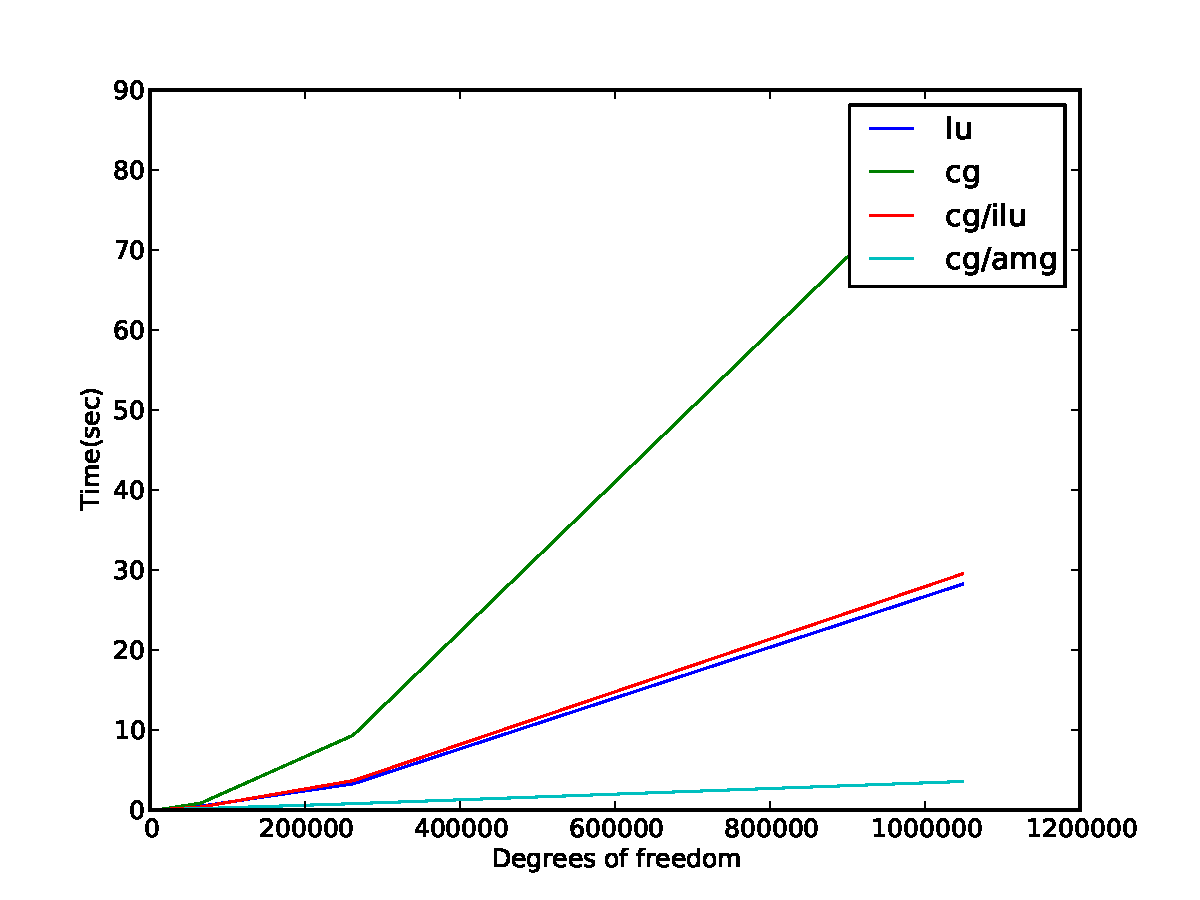
\includegraphics[width=8cm, height=7cm]{chapters/iterative_methods/plots/cpu_time_comparison_plot.pdf}
\caption{CPU time (in seconds) for solving a linear system of equation with $N$ degrees of freedom (x-axis) 
             for different solvers} 
\label{fig:CPU_time}
\end{figure}

\begin{python}
from dolfin import *
import time
lu_time = []; cgamg_time = []
cg_time = []; cgilu_time = []
Ns = []

parameters["krylov_solver"]["relative_tolerance"] = 1.0e-8
parameters["krylov_solver"]["absolute_tolerance"] = 1.0e-8
parameters["krylov_solver"]["monitor_convergence"] = False
parameters["krylov_solver"]["report"] = False
parameters["krylov_solver"]["maximum_iterations"] = 50000

def solving_time(A,b, solver):
  U = Function(V)
  t0 = time.time()
  if len(solver) == 2: 
    solve(A, U.vector(), b, solver[0], solver[1]);
  else: 
    solve(A, U.vector(), b, solver[0]);
  t1 = time.time()
  return t1-t0

for N in [32, 64, 128, 256, 512, 1024]:

  Ns.append(N)

  mesh = UnitSquare(N, N)
  print " N ", N, " dofs ", mesh.num_vertices()
  V = FunctionSpace(mesh, "Lagrange", 1)
  u = TrialFunction(V)
  v = TestFunction(V)

  f = Expression("sin(x[0]*12) - x[1]")
  a = u*v*dx  + inner(grad(u), grad(v))*dx
  L = f*v*dx

  A = assemble(a)
  b = assemble(L)
  
  t2 = solving_time(A,b, ["lu"])
  print "Time for lu ", t2
  lu_time.append(t2)
  
  t2 = solving_time(A, b, ["cg"])
  print "Time for cg ", t2
  cg_time.append(t2)

  t2 = solving_time(A, b, ["cg", "ilu"])
  print "Time for cg/ilu ", t2
  cgilu_time.append(t2)

  t2 = solving_time(A, b, ["cg", "amg"])
  print "Time for cg/amg ", t2
  cgamg_time.append(t2)


import pylab

pylab.plot(Ns, lu_time)
pylab.plot(Ns, cg_time)
pylab.plot(Ns, cgilu_time)
pylab.plot(Ns, cgamg_time)  
pylab.xlabel('Unknowns')
pylab.ylabel('Time(sec)')
pylab.legend(["lu", "cg", "cg/ilu", "cg/amg"])
pylab.show()

pylab.loglog(Ns, lu_time)
pylab.loglog(Ns, cg_time)
pylab.loglog(Ns, cgilu_time)
pylab.loglog(Ns, cgamg_time)
pylab.legend(["lu", "cg", "cg/ilu", "cg/amg"])
pylab.savefig('tmp_cpu.pdf')
pylab.show()
\end{python}
\end{example}

When we employ iterative methods, we need to specify the convergence criterion. This is often 
not an easy task. We have the continuous solution $u$, the discrete solution $u_h$, and the
appropriate discrete solution, $u_h^n$ found by an iterative method at iteration $n$.  
Obviously, we may estimate the error as
\[
\|u-u^n_h\| \le \|u-u_h\| + \|u_h-u_h^n\|, 
\]
and it does make sense that the values of 
$\|u-u_h\|$ and $\|u_h-u_h^n\|$ are balanced. Still both terms may be hard to estimate in 
challenging applications. In practice, an appropriate convergence criterion is usually 
found by trial and error by choosing a stopping criterion based on the residual.   
Let us therefore consider a concrete example and consider $\|u-u^n_h\|$ 
as a function of the mesh resolution and a varying convergence criterion. 


\begin{table}
\begin{tabular}{c|ccccc}
\hline 
$\epsilon\backslash$ N & 64 & 128 & 256 & 512 & 1024 \\ \hline 
1.0e-1 &  1.3e-02 (1.1e-02) &  1.4e-02 (3.5e-02) &  8.8e-03 (1.4e-01) &  3.4e-03 (5.9e-01) &  1.1e-02 (2.5e+00) \\ 
1.0e-2 &  1.2e-03 (1.0e-02) &  2.0e-03 (3.7e-02) &  1.3e-03 (1.5e-01) &  3.5e-03 (5.8e-01) &  3.7e-04 (2.7e+00) \\ 
1.0e-3 &  3.6e-04 (1.1e-02) &  3.1e-04 (3.9e-02) &  2.6e-04 (1.6e-01) &  2.7e-04 (6.3e-01) &  3.7e-04 (2.7e+00) \\ 
1.0e-4 &  3.4e-04 (1.2e-02) &  8.5e-05 (4.5e-02) &  2.4e-05 (1.8e-01) &  3.4e-05 (6.7e-01) &  1.4e-05 (2.9e+00) \\ 
1.0e-5 &  3.4e-04 (1.2e-02) &  8.4e-05 (4.7e-02) &  2.1e-05 (1.9e-01) &  5.4e-06 (7.6e-01) &  2.8e-06 (3.1e+00) \\ 
1.0e-6 &  3.4e-04 (1.3e-02) &  8.4e-05 (5.0e-02) &  2.1e-05 (2.1e-01) &  5.3e-06 (8.1e-01) &  1.3e-06 (3.3e+00) \\ 
\end{tabular}
\caption{The error $\|u-u^n_h\|$ and corresponding CPU time in parentesis when solving a Poisson problem
with homogenuous Dirichlet conditions. } 
\label{conv:res:error}. 
\end{table}



Table \ref{conv:res:error} shows the error and the corresponding CPU timings when solving a Poisson problem
at various resolutions and convergence criteria. 
Here, the convergence criteria is chosen as reducing the relative residual, i.e., $\frac{\|r_k\|}{\|r_0\|}$
by the factor $\epsilon$. This convergence criteria is very common, in particular for stationary problems.  
There are several things to note here. For coarse resolution, \emp{N=64}, the error stagnates somewhere
between $1.0e-3$ and $1.0e-4$ and this stagnation marks where an appropriate stopping criteria is.   
It is however worth noticing that solving it to a criteria that is 
$1.0e-6$ is actually only about 30\% more computationally demanding than $1.0e-3$. This is due to the
fact that we have a very efficient method that reduces the error by about a factor 10 per iteration.   
If we consider the fine resolution, \emp{N=1024}, we see that the stagnation happens later and that
we may not even have reached the stagnating point even at $\epsilon=1.0e-6$. We also notice that 
the decreasing $\epsilon$ in this case only lead to a moderate growth in CPU time.   
If we look closer at the table, we find that the stagnation point follows a staircase pattern. 
The code used to generate the table is as follows: 

\begin{python}
from dolfin import *

def boundary(x, on_boundary):
    return on_boundary

parameters["krylov_solver"]["relative_tolerance"] = 1.0e-18 
parameters["krylov_solver"]["absolute_tolerance"] = 1.0e-18 
parameters["krylov_solver"]["monitor_convergence"] = True 
parameters["krylov_solver"]["report"] = True 
#parameters["krylov_solver"]["maximum_iterations"] = 50000 
epss = [1.0e-1, 1.0e-2, 1.0e-3, 1.0e-4, 1.0e-5, 1.0e-6]
data = {}
Ns= [64, 128, 256, 512, 1024]
#Ns= [8, 16, 32, 64]
for N in Ns:
  for eps in epss:  
    parameters["krylov_solver"]["relative_tolerance"] = eps 

    mesh = UnitSquareMesh(N, N)
    V = FunctionSpace(mesh, "P", 1)
    u = TrialFunction(V)
    v = TestFunction(V)

    u_ex = Expression("sin(3.14*x[0])*sin(3.14*x[1])", degree=3) 
    f = Expression("2*3.14*3.14*sin(3.14*x[0])*sin(3.14*x[1])", degree=3) 
    a = inner(grad(u), grad(v))*dx  
    L = f*v*dx 

    U = Function(V)

    A = assemble(a) 
    b = assemble(L)

    bc = DirichletBC(V, u_ex, boundary)
    bc.apply(A)
    bc.apply(b) 

    t0 = time()
    solve(A, U.vector(), b, "gmres", "amg")
    t1 = time()

    cpu_time = t1-t0
    error_L2 = errornorm(u_ex, U, 'L2', degree_rise=3)
    data[(N, eps)] = (error_L2, cpu_time) 

for eps in epss:  
  for N in Ns:
    D1, D2 = data[(N, eps)]
    print " %3.1e (%3.1e) " % (D1, D2), 
    print ""
	
\end{python}

\begin{example}{\textbf{Eigenvalues of the preconditioned system.}}
It is often interesting to assess the condition number of the 
preconditioned system, $BA$. If the preconditioner is a matrix and the
size of the system is moderate we may be able to estimate the condition
number of $BA$ using NumPy, Matlab or Octave. However, when our preconditioner
is an algorithm representing a linear operator, such as in the case
of multigrid, then this is not possible. However, as described in~\cite{saad2003iterative}, 
egenvalues may be estimated as a bi-product of the Conjugate Gradient method. Without
going into the algorithmic details of the implmementation, we mention that
this is implemented in the FEniCS module \emp{cbc.block}, see~\cite{mardal2012block}.      
The following code shows the usage.  
\begin{python}
from dolfin import *
from block.iterative import ConjGrad
from block.algebraic.petsc import ML
from numpy import random

def boundary(x, on_boundary):
    return on_boundary

class Source(Expression):
    def eval(self, values, x):
        dx = x[0] - 0.5; dy = x[1] - 0.5
        values[0] = 500.0*exp(-(dx*dx + dy*dy)/0.02)

Ns = [8, 16, 32, 64, 128, 256, 512, 1024]
for N in Ns: 
    mesh = UnitSquareMesh(N,N)
    V = FunctionSpace(mesh, "CG", 1)

    # Define variational problem
    v = TestFunction(V)
    u = TrialFunction(V)
    f = Source(degree=3)
    a = dot(grad(v), grad(u))*dx
    L = v*f*dx 
    bc = DirichletBC(V, Constant(0), boundary)

    # Assemble matrix and vector, create precondition and start vector 
    A, b = assemble_system(a,L, bc)
    B = ML(A)
    x = b.copy()
    x[:] = random.random(x.size(0))

    # solve problem and print out eigenvalue estimates. 
    Ainv = ConjGrad(A, precond=B, initial_guess=x, tolerance=1e-8, show=2)
    x = Ainv*b
    e = Ainv.eigenvalue_estimates()
    print "N=%d iter=%d K=%.3g" % (N, Ainv.iterations, e[-1]/e[0])
\end{python}
In this example we see that the condition number increases logaritmic from 1.1 to 2.1 as the \emp{N}
increases from 8 to 1024. The \emp{AMG} preconditioner has better performance and does
not show logaritmic growth. For indefinite symmetric systems, the \emp{CGN} method provides
the means for estimating the condition number, c.f., the \emp{cbc.block} documentation.    
\end{example}

\subsection{Insight from Functional Analysis}
In the previous Chapters \ref{chap-conv} and \ref{chap-stokes}
we have discussed the well-posedness of the convection-diffusion
equations and the Stokes problem. In both cases, the problems 
were well-posed - meaning that the differential operators
as well as their inverse were continuous. 
However, when we discretize the problems we get matrices
where the condition number grows to infinity as the element size goes to  
zero. This seem to contradict the well-posedness of our discrete problems
and may potentially destroy both the accuracy and efficiency 
of our numerical algorithms. Functional analysis explains this 
apparent contradiction and explains how the problem is circumvented by 
preconditioning.   

Let us now consider the seeming contradiction in more precise
mathematical detail for the Poisson problem 
with homogeneous Dirichlet conditions:  
Find $u$ such that 
\begin{eqnarray}
- \Delta u &=& f, \quad \text{ in } \Omega,  \\     
u &=& 0, \quad \text{ on } \partial \Omega .  
\end{eqnarray}

We know from Lax-Milgram's theorem that 
the weak formulation of this problem: 
Find $u\in H^1_0$ such that 
\[
a(u, v) = b(v), \quad \forall v\in H^1_0 .   
\]
where 
\begin{eqnarray}
a(u,v) &=& \int_\Omega \nabla u \cdot \nabla v \, dx, \\   
b(v)   &=& \int_\Omega  f  v \, dx,   
\end{eqnarray}
is well-posed because 
\begin{eqnarray}
a(u,u) &\ge& \alpha |u|^2_{1} \ , \quad \forall u \in H^1_0  \\ 
a(u,v) &\le& C |u|_{1} |v|_{H_0^1} \quad \forall u,v \in H^1_0   \ . 
\end{eqnarray}
Here $|\cdot|_{1}$ denotes the $H^1$ semi-norm which is known to 
be a norm on $H^1_0$ due to Poincare.  
The well-posedness is in this case stated as
\begin{equation}
|u|_{H_0^1} \le \frac{1}{\alpha} \|f\|_{H^{-1}} .  
\end{equation}
In other words, $-\Delta$ takes a function $u$ in $H^1_0$ and  
returns a function $f=-\Delta u$ which is in $H^{-1}$. We
have that $\|f\|_{-1} = \|-\Delta u\|_{-1} \le C \|u\|_1$.     
Also, $-\Delta^{-1}$ takes a function $f$ in $H^{-1}$ and  
returns a function $u=(-\Delta)^{-1} f$ which is in $H^1_0$. We
have that $\|u\|_{1} = \|(-\Delta)^{-1} f\|_{1} \le \frac{1}{\alpha} \|f\|_{-1}$.     
In fact, in this case $\alpha=C=1$. 

This play with words and symbols may be formalized by using operator norms that
are equivalent with matrix norms. Let $B \in \R^{n,m}$ then
\[    
\|B\|_{\mathcal{L}(\R^m, \R^n)} = \max_{x\in\R^m} \frac{\Vert B x\Vert_{\R^n}}{\Vert x \Vert_{\R^m}}   
\]
Here $\mathcal{L}(\R^m, \R^n)$ denotes the space of all $m\times n$ matrices. 

Analogously, we may summarize the mapping properties of $-\Delta$ and  $(-\Delta)^{-1}$ 
in terms of the conditions of Lax-Milgram's theorem as  
\begin{equation} 
\label{boundeddelta}
\|-\Delta\|_{\mathcal{L}(H^1_0, H^{-1})} \le C
\quad \text{ and } \quad  
\|(-\Delta)^{-1}\|_{\mathcal{L}(H^{-1}, H^1_0) } \le \frac{1}{\alpha} \ . 
\end{equation}
where ${\mathcal{L}(X, Y)}$ denotes the space of bounded linear operators mapping
$X$ to $Y$.  
In other words, $-\Delta$ is a bounded linear map from
$H^1_0$ to $H^{-1}$ and 
$(-\Delta)^{-1}$ is a bounded linear map from
$H^{-1}$ to $H^1_0$. 
This is a crucial observation
in functional analysis that, in contrast to the case of  
a matrix which is  a bounded linear map from $\R^n$ to $\R^m$, 
an operator may be map from one space to another. 

From Chapter \ref{chap-sobolev} we know that the eigenvalues
and eigenvectors of $-\Delta$ with homogeneous Dirichlet
conditions on the unit interval in 1D are
$\lambda_k=(\pi k)^2$ and $e_k = sin(\pi k x)$, respectively. 
Hence the eigenvalues of $-\Delta$ obviously tend to $\infty$
as $k$ grows to $\infty$ and similarly the eigenvalues
of $(-\Delta)^{-1}$ accumulate at zero as $k\rightarrow \infty$.  
Hence the spectrum of $-\Delta$ is unbounded and the 
spectrum of $(-\Delta)^{-1}$ has an accumulation point at zero.  
Still, the operator $-\Delta$ and its inverse are bounded
from a functional analysis point of view, in the sense of 
\eqref{boundeddelta}.  


Let us for the moment assume that we have access to an operator $B$ with mapping
properties that are inverse to that of $A=-\Delta$, i.e., 
\begin{equation} 
\label{boundedB}
\|B\|_{\mathcal{L}(H^{-1}, H^1_0) } \  
\quad \text{ and } \quad  
\|B^{-1}\|_{\mathcal{L}(H^1_0, H^{-1})} . 
\end{equation}
Then it follows directly that 
\begin{equation} 
\label{boundeddelta}
\|B A\|_{\mathcal{L}(H^1_0, H^1_0) } \  
\quad \text{ and } \quad  
\|(B A)^{-1}\|_{\mathcal{L}(H^1_0, H^1_0)} . 
\end{equation}
and the condition number 
\[
\kappa(BA) = \frac{\max_i \lambda_i (BA)}{\min _i \lambda_i (BA)} =    \|B A\|_{\mathcal{L}(H^1_0, H^1_0) }   \|(B A)^{-1}\|_{\mathcal{L}(H^1_0, H^1_0)}
\]
would be bounded.  
In the discrete case, the mapping property \eqref{boundedB} translates to the fact that  $B$ should be spectrally equivalent with the inverse of $A$ 
when $B$ and $A$ are both positive.  

While the above discussion is mostly just a re-iteration of the concept of spectral equivalence in the discrete case 
when the PDEs are elliptic, 
the insight from functional analysis can be powerful for systems of PDEs. 
Let us consider the Stokes problem from Chapter \ref{chap-stokes}.  
The problem reads: 
\[
\mathcal{A}  
\left[ 
\begin{array}{c}
u \\ p  
\end{array}
\right]
=
\left[ 
\begin{array}{cc}
-\Delta & -\nabla \\  
\nabla\cdot & 0  
\end{array}
\right]
\left[ 
\begin{array}{c}
u \\ p  
\end{array}
\right]
=
\left[ 
\begin{array}{c}
u \\ p  
\end{array}
\right]
\]
As discussed in Chapter \ref{chap-stokes} 
\[
\mathcal{A} : H^1_0 \times L^2 \rightarrow   H^{-1} \times L^2 
\]
was a bounded linear mapping with a bounded inverse.  
Therefore, a preconditioner can be constructed as 
\[
\mathcal{B}
= 
\left[ 
\begin{array}{cc}
(-\Delta)^{-1} & 0 \\  
0 & I  
\end{array}
\right]
\]
Clearly 
\[
\mathcal{B}:  H^{-1} \times L^2 \rightarrow H^1_0 \times L^2   
\]
and is therefore a suitable preconditioner. However, we also notice that
$\mathcal{A}$ and $\mathcal{B}^{-1}$ are quite different. 
$\mathcal{A}$ is indefinite and has positive and negative egenvalues, while
$\mathcal{B}$ is clearly positive. Hence, the operators are not spectrally equivalent.    
Exercise \ref{ex:stokes} looks deeper into this construction of preconditioners
for Stokes problem. A more comprehensive description of this technique
can be found in \cite{mardal2011preconditioning}.



\section{Exercises}

\begin{exercise}
\label{ex:nnz}
Estimate ratio of non-zeros per unknown of the stiffness matrix on the unit square   
with Lagrangian elements of order 1, 2, 3 and 4. Hint: the 
number of non-zeros can be obtained from the function 'nnz' of a matrix object.  
\end{exercise}

\begin{exercise}
\label{ex:eig:1D2D3D}
Compute the smallest and largest eigenvalues of the mass matrix and 
the stiffness matrix in 1D, 2D and 3D. Assume that
the condition number is on the form  
$\kappa \approx C h^\alpha$, where $C$ and $\alpha$ may
depend on the number of dimentions in space.   
Finally, compute the corresponding condition numbers.  
Does the condition number have the same dependence on 
the number of dimentions in space?  
\end{exercise}

\begin{exercise}
\label{ex:eig:1D2D3D:order}
Repeat Exercise \ref{ex:eig:1D2D3D} but with Lagrange elements of order 1, 2 and 3.  
How does the order of the polynomial affect the eigenvalues and condition numbers. 
\end{exercise}


\begin{exercise}
Compute the eigenvalues the discretized Stokes problem
using Taylor-Hood elements. Note that the problem
is indefinite and that there are both positive and 
negative eigenvalues. An appropriate condition number
is:   
\[
\kappa = \frac{ \max_i |\lambda_i |}{ \min_i | \lambda_i|}
\]
where $\lambda_i$ are the eigenvalues of $A$. 
Compute corresponding condition numbers for the Mini and Crouzeix-Raviart 
elements. Are the condition numbers similar?  
\end{exercise}

\begin{exercise}
Implement the Jacobi iteration for a 1D Poisson problem with homogeneous
Dirichlet conditions. Start the iteration with an initial random vector and
estimate the number of iterations required to reduce the $L_2$ norm of the  residual
with a factor $10^4$. For relevant code see Example \ref{example:CPU_time}.
\end{exercise}


\begin{exercise}
\label{ex:poisson}
Test CG method without preconditioer, with ILU preconditioner and with AMG preconditioner 
for the Poisson problem in 1D and 2D with homogeneous Dirichlet conditions,  with respect
to different mesh resolutions. Do some of the iterations suggest spectral equivalence?
\end{exercise}

\begin{exercise}
\label{ex:conv}
Test CG, BiCGStab, GMRES with ILU, AMG, and Jacobi preconditioning for 
\begin{eqnarray*}
-\mu\Delta u + v\nabla u   &=& f \quad \textrm{in}\ \Omega\\
u&=& 0 \quad \textrm{on}\ \partial\Omega
\end{eqnarray*}
Where $\Omega$ is the unit square, $v=c\, sin(7 x)$, and $c$ varies as $1, 10, 100, 1000, 10 000$ and
the mesh resolution $h$ varies as $1/8, 1/16, 1/32, 1/64$. You may assume homogeneous Dirichlet conditions.  

\end{exercise}



\begin{exercise}
\label{ex:stokes}
The following code snippet shows the assembly of the matrix and preconditioner
for a Stokes problem: 
\begin{python} 
a = inner(grad(u), grad(v))*dx + div(v)*p*dx + q*div(u)*dx
L = inner(f, v)*dx

# Form for use in constructing preconditioner matrix
b = inner(grad(u), grad(v))*dx + p*q*dx

# Assemble system
A, bb = assemble_system(a, L, bcs)

# Assemble preconditioner system
P, btmp = assemble_system(b, L, bcs)

# Create Krylov solver and AMG preconditioner
solver = KrylovSolver("tfqmr", "amg")

# Associate operator (A) and preconditioner matrix (P)
solver.set_operators(A, P)

# Solve
U = Function(W)
solver.solve(U.vector(), bb)
\end{python} 
Here, "tfqmr" is a variant of the Minimal residual method and "amg" is an algebraic 
multigrid implementation in HYPRE. Test, by varying the mesh resolution, whether
the code produces an order--optimal preconditioner.  
HINT: You might want to change the "parameters" as done
in Example \ref{example:CPU_time}: 
\begin{python}
# Create Krylov solver and AMG preconditioner
solver = KrylovSolver("tfqmr", "amg")
solver.parameters["relative_tolerance"] = 1.0e-8
solver.parameters["absolute_tolerance"] = 1.0e-8
solver.parameters["monitor_convergence"] = True
solver.parameters["report"] = True
solver.parameters["maximum_iterations"] = 50000
\end{python}
\end{exercise}

\begin{exercise}
\label{ex:stokes}
Consider the mixed formulation of linear elasticity that
is appropriate when $\lambda$ is large compared to $\mu$. That is, 
\begin{python} 
a = inner(grad(u), grad(v))*dx + div(v)*p*dx + q*div(u)*dx - 1/lam*p*q*dx 
L = inner(f, v)*dx
\end{python}
Create two preconditioners: 
\begin{python} 
b1 = inner(grad(u), grad(v))*dx + p*q*dx
b2 = inner(grad(u), grad(v))*dx + 1/lam*p*q*dx
\end{python} 
Compare the efficiency of the different preconditioners when increasing
the resolution and when $\lambda\rightarrow\infty$. 
Can you explain why the first preconditioner is the best?
\end{exercise}



%Suggestions to exercise:
%Show that the eigenvalues to the Jacobi(and relaxed) are ...
%Show/prove the "show this" 

%------------------------------------------------------------------------------

%Triks fra Adrian
%\begin{align}
%Lu =&\left\{ \begin{array}{lr}  -u(x)'' &= f(x) \quad \foralls x \in \Omega\\ u(0) = u(1) &= 0  \end{array}% \right. \end{align}
